\documentclass[11pt]{article}
\usepackage{amsfonts}
\usepackage{amsmath}
\usepackage{amssymb}
\usepackage{amsthm}
\usepackage{latexsym}
\usepackage[mathscr]{eucal}
\usepackage{natbib}
\usepackage{graphicx}
\usepackage{xcolor}
\usepackage[spanish]{babel}
\usepackage[utf8]{inputenc}


\setlength{\parindent}{2em}
\setlength{\parskip}{2mm}
\textheight = 220mm
\textwidth 152mm
\oddsidemargin 5mm
\evensidemargin 5mm
\topmargin -5mm


\begin{document}
\begin{center}
\textcolor{blue}{{\LARGE \textbf{Modelo para el Trabajo de los Temas 6 y 7 de\\[3mm] Inferencia Estadística }}}\\[3mm]
\Large{Curso 2020/2021 \\[3mm]
Autores/as del trabajo }
\end{center} 


\section{Indicaciones}
Esta es una plantilla diseñada en MS Word para poder redactar el trabajo de evaluación continua correspondiente a los Temas 6 y 7 de la materia de Inferencia Estadística.

A lo largo del presente documento debes responder de manera razonada a las diferentes cuestiones que se proponen en el enunciado de la tarea que puedes encontrar en el Campus Virtual. Dichas explicaciones deberán apoyarse en los resultados obtenidos con el programa estadístico R.

Además, también deberás incluir en este informe el código empleado para obtener los resultados y las representaciones gráficas obtenidas. Podrías añadir el código y los diferentes resultados de la siguiente forma:
\begin{verbatim}
> set.seed(1234)
> x=rnorm(100)
> mean(x)
[1] -0.1567617
> var(x)
[1] 1.00883
\end{verbatim}


Por otra parte, trabajando con \LaTeX\, es muy sencillo incluir ecuaciones:
$$
\begin{cases}
H_0: \beta_1=0,\\
H_a: \beta_1\neq 0
\end{cases}
$$
o tablas:
\begin{center}
\begin{tabular}{ |c c c| }
 \hline
 celda1 & celda2 & celda3 \\
 \hline \hline
 celda4 & celda5 & celda6 \\  
 celda7 & celda8 & celda9 \\   
  \hline
\end{tabular}
\end{center}

\subsection{Incluir representaciones gráficas}
Finalmente, si en el informe deseas incorporar alguna representación gráfica, puedes emplear la sintaxis de la Figura \ref{etiqueta}.
\begin{figure}
\begin{center} 
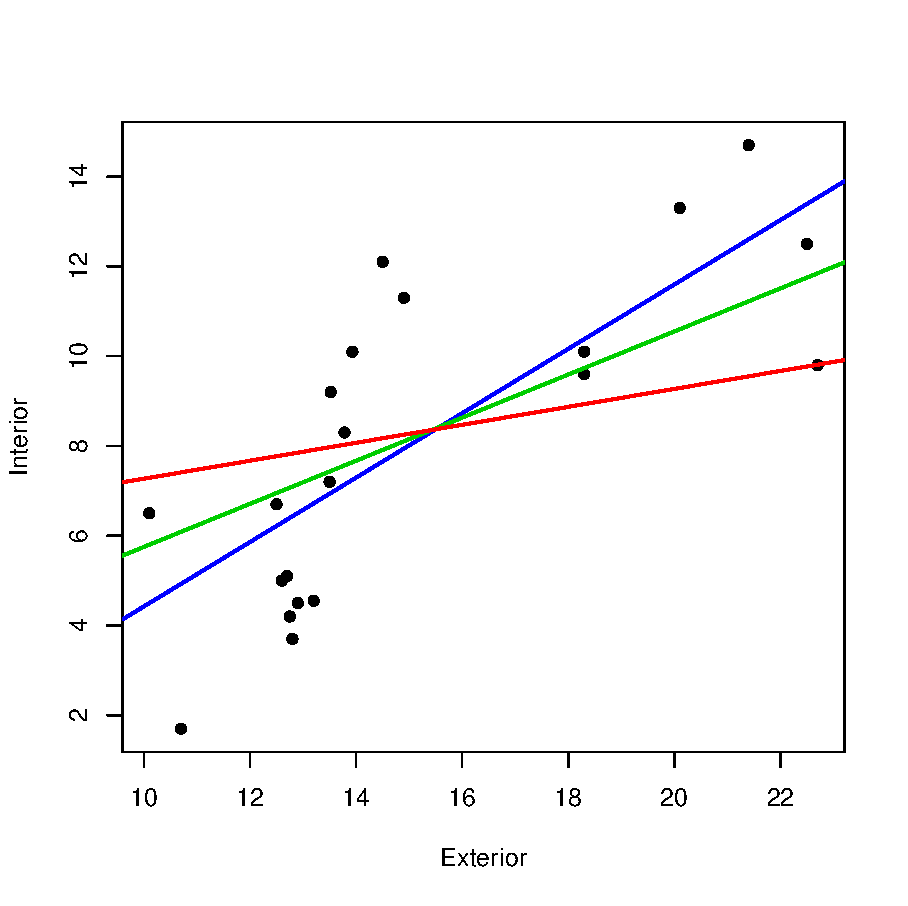
\includegraphics[scale=0.5]{exemplo-figura.pdf} 
\end{center} 
\caption{Pie de figura.}
\label{etiqueta}
\end{figure}

\end{document}